\documentclass[11pt,letterpaper]{article}
\usepackage[T1]{fontenc}
\usepackage[utf8]{inputenc}
\usepackage[scaled=0.95]{helvet}
\renewcommand{\familydefault}{\sfdefault}
\usepackage[letterpaper,top=0.9in,bottom=0.95in,left=1in,right=1in]{geometry}
\usepackage{microtype}
\usepackage{enumitem}
\usepackage{titlesec}
\usepackage{fancyhdr}
\usepackage{xcolor}
\usepackage{booktabs}
\usepackage{array}
\usepackage{graphicx}
\usepackage{textcomp}
\usepackage[hidelinks]{hyperref}
\urlstyle{same}
\newcommand{\docversion}{2026-10-23-10-21-40} % set by build.py (America/Toronto)
\hypersetup{pdfsubject={version \docversion},pdftitle={Les déclarations de bienfaisance (T3010) de la paroisse St Monica, 2008 à 2024 : données, méthode et chiffres}}

\setlength{\parindent}{0pt}
\setlength{\parskip}{0.5em}
\linespread{1.03}
\sloppy
\titleformat{\section}{\normalfont\large\bfseries}{\thesection}{0.6em}{}[\vspace{1pt}\titlerule]
\titlespacing*{\section}{0pt}{1.1em}{0.4em}
\titleformat{\subsection}{\normalfont\bfseries}{\thesubsection}{0.6em}{}
\titlespacing*{\subsection}{0pt}{0.8em}{0.25em}
\pagestyle{fancy}
\fancyhf{}
\renewcommand{\headrulewidth}{0pt}
\fancyfoot[C]{\footnotesize\color{gray}Paroisse St Monica, déclarations T3010 -- note de données -- page \thepage}
\fancyfoot[R]{\tiny\color{gray}v.\,\docversion}
\renewcommand{\tablename}{Tableau}
\newcommand{\repourl}{https://github.com/OpenMobilityData/Terrebonne-open-sources}
\newcommand{\folder}{2024-st-monica-cra-t3010}
\newcommand{\D}[1]{#1\,\$}

\begin{document}

{\LARGE\bfseries Les déclarations de bienfaisance (T3010) de la paroisse St Monica, 2008 à 2024}\par\medskip
{\large Données, méthode et chiffres}\par\medskip
{\small Un résident de Côte-des-Neiges--Notre-Dame-de-Grâce, à partir de documents publics. Version \docversion. Dépôt~: \href{\repourl}{\repourl}, dossier \texttt{\folder}. Version française de la note \texttt{st\_monica\_t3010\_note\_en.pdf}~; en cas d'écart, le texte anglais et les tables font foi.}

\section*{Résumé}

\textbf{Hypothèse examinée.} Que la piste cyclable protégée aménagée sur la rue de Terrebonne en mai--juin 2024 a eu un effet mesurable sur les finances de la paroisse. \textbf{Matériel.} La section financière publique des dix-sept déclarations T3010 de la paroisse, exercices 2008 à 2024 (années civiles), telles que communiquées par l'ARC. La déclaration de 2024 est la seule dont l'année comprend la piste, pour ses sept derniers mois~; celle de 2025, première année complète, n'était pas encore publiée le 23~octobre 2026. \textbf{Ce que montre la déclaration de 2024.} Des revenus totaux de \D{250\,718}, dans la fourchette des cinq années précédentes (\D{202\,900} à \D{276\,981}), 6~\% sous 2023 et 4~\% sous 2022, au-dessus de 2020 et 2021. Sur les lignes de revenus les plus proches des affirmations entendues dans le débat~: dons avec reçu \D{201\,562}, 2~\% sous 2023 et au-dessus de 2020, 2021 et 2022~; autres dons sans reçu \D{18\,311}, sous 2022 et 2023 et au-dessus de 2020 et 2021~; revenus de location \D{15\,339}, au niveau de 2022 et 2023~; «\,autres revenus\,» (la ligne qui nommait messes, funérailles et mariages en 2011) \D{15\,506}, plus élevés que toute année depuis 2014, mais décrits dans la déclaration de 2024 comme frais de catéchèse et lampions, non comme funérailles ou mariages. La déclaration n'a pas de ligne pour les mariages ni les funérailles~; la ligne qui les a portés est presque vide depuis 2015, et les sommes versées à ces occasions peuvent figurer sur quatre lignes différentes selon la pratique de la paroisse (section~\ref{sec:4650}). Des dépenses de \D{269\,373} ont dépassé les revenus de \D{18\,655}, troisième année consécutive de dépenses supérieures aux revenus après 2022 (\D{31\,771}) et 2023 (\D{8\,240}), et septième des dix-sept années~; la hausse de cet écart de 2023 à 2024 (\D{10\,415}) est inférieure à la hausse de la ligne de rémunération (\D{15\,783}). L'encaisse et les placements à court terme ont monté à \D{197\,111} et le total du passif à \D{180\,109}, l'un le plus élevé depuis 2011, l'autre le plus élevé de la série. \textbf{Conclusion.} La déclaration de 2024 ne montre aucun chiffre qui se détache de la variation d'une année à l'autre de 2019--2023, au cours de laquelle les dons avec reçu ont bougé de 2 à 15~\% entre années consécutives et les revenus totaux de 3 à 28~\%~; les déficits précèdent la piste. Contre les douze autres paroisses catholiques des mêmes secteurs postaux (section~\ref{sec:peers}), la variation de la paroisse de 2023 à 2024 ($-$6~\% sur les dons, $-$6~\% sur le total des revenus) se situe sous la médiane des voisines ($+$1~\% et $+$5~\%) et à l'intérieur de la moitié centrale de leurs variations~; l'écart de la paroisse à la médiane des voisines s'est ouvert en 2023, avant la piste. \textbf{Seuil de détection.} Compte tenu de la variation d'une année à l'autre observée de 2015 à 2023, on ne peut attendre de ce dossier qu'il détecte un changement lié à la piste dans les dons de la paroisse inférieur à environ 15 à 26~\% des dons d'une année contre l'histoire de la paroisse elle-même, ou à environ 14 à 16 points contre la variation médiane des douze paroisses voisines (deux écarts-types des variations d'avant la piste, le chiffre le plus bas sans les trois transitions COVID~; section~\ref{sec:threshold}). Comme la piste a couvert sept des douze mois de 2024, un effet de la piste aurait dû retrancher environ 25 à 45~\% des dons annuels de la paroisse, et environ 21 à 50~\% de ses revenus totaux, pour se détacher dans la déclaration de 2024~; les variations observées en 2024 ($-$6,1~\% sur les dons, $-$6,9 points contre les voisines) sont bien en deçà de ces seuils. La déclaration de 2025, une année complète, abaisserait le seuil à environ 14 à 26~\% des dons, et deux années complètes à environ 10 à 18~\%.
 Un effet mesurable n'est donc ni établi ni exclu par ce dossier~: il aurait dû être grand, de l'ordre du quart des dons d'une année, pour paraître dans la déclaration de 2024. Ce qui permettrait un test plus fort~: la déclaration de 2025, lue de la même façon contre les voisines~; et des chiffres mensuels, que la paroisse a publiés dans ses bulletins jusqu'en mars 2023 et plus depuis (section~\ref{sec:statements}~; là où état et déclaration se comparent, 2019, 2020 et 2022, ils concordent au dollar près).

\section{Objet et portée}

La paroisse St Monica (La fabrique de la paroisse de Sainte-Monique, 6405, rue de Terrebonne) est un organisme de bienfaisance enregistré. Comme tout organisme enregistré au Canada, elle produit chaque année une déclaration de renseignements, le formulaire T3010, auprès de l'Agence du revenu du Canada (ARC), et la section financière de cette déclaration est publique. Le bâtiment de la paroisse se trouve sur la rue de Terrebonne, sur le tronçon où une piste cyclable protégée a été aménagée en 2024, et la situation de la paroisse a été évoquée dans le débat public sur cette piste. La présente note documente les déclarations de la paroisse telles que l'ARC les a communiquées, explique comment les tables et les graphiques du dossier en sont tirés, et lit les graphiques dans les termes de la déclaration elle-même. Elle n'attribue aucun chiffre à aucune cause~: les déclarations ne portent pas cette information.

Les données couvrent les exercices clos le 31~décembre, de 2008 à 2024~: dix-sept déclarations. Les années 2008 à 2018 proviennent d'une demande de données à laquelle l'ARC a répondu le 6~décembre 2024~; les années 2019 à 2024 sont des extraits de lignes des fichiers de données ouvertes annuels de l'ARC, téléchargés le 23~octobre 2026 (section~\ref{sec:prov}). Une transcription des années 2019 à 2023, faite à la fin de 2024 à partir de l'«\,aperçu\,» de la Liste des organismes de bienfaisance de l'ARC, a servi de source provisoire jusque-là~; elle a été vérifiée contre les fichiers puis retirée (section~\ref{sec:interim}). La déclaration de 2024 est la première dont l'exercice comprend les mois qui suivent l'aménagement de la piste (mai--juin 2024)~; la déclaration de 2025 n'était pas encore publiée le 23~octobre 2026.

\section{La déclaration T3010}

Le formulaire T3010 comporte une section financière (section~D pour les organismes qui déclarent sur le formulaire abrégé, annexe~6 pour les autres) dont les entrées sont numérotées. Les numéros employés ici sont les numéros de ligne de l'ARC~; les libellés sont dans \texttt{derived/line\_labels.csv} avec une colonne de statut~: \emph{checked} lorsque le sens de la ligne est confirmé par les données en main (un total qui s'additionne, une ligne de texte qui nomme son contenu, un chiffre qui concorde avec le bilan publié par la paroisse), \emph{dictionary} lorsque le libellé est celui du dictionnaire de données de l'ARC (\emph{List of charities data dictionary}, version 2.0, conservé avec le jeu de données 2024 dans \texttt{raw/open-canada/references/}), \emph{quick\_view} lorsqu'il reprend le texte de la page de la Liste des organismes tel que transcrit en 2024, \emph{form} lorsque le libellé est pris du formulaire sans confirmation indépendante. L'ARC publie le formulaire et son guide (T4033) sur canada.ca. La version 27 du formulaire, employée pour les exercices 2023 et 2024, ajoute des sous-lignes qui reprennent une partie d'une ligne existante (4101, argent comptant et comptes bancaires inclus à la 4100~; 4157, terrains et immeubles utilisés pour les activités de l'organisme, inclus à la 4155~; 4576, revenus d'investissements d'impact inclus à la 4580)~; elles sont conservées dans la table longue et ne sont ajoutées à aucun total.

Les lignes employées dans les figures sont~:
\begin{itemize}[nosep,leftmargin=1.4em]
\item \textbf{4700} total des revenus~; \textbf{4500} montant admissible total des dons pour lesquels l'organisme a délivré des reçus~; \textbf{4530} autres dons (sans reçu)~; \textbf{4650} autres revenus non compris ailleurs, que la ligne 4655 décrit en 2011 comme «\,Masses, funeral, weddings etc\,»~; \textbf{4610} revenu brut de location de terrains ou d'immeubles~; \textbf{4580} intérêts et revenus de placements~; \textbf{4540}, \textbf{4550}, \textbf{4560} revenus des gouvernements fédéral, provincial et municipal~;
\item \textbf{5100} total des dépenses~; \textbf{4880} total de la rémunération~; \textbf{4850} frais d'occupation~; \textbf{4840} fournitures et frais de bureau~; \textbf{4860} honoraires professionnels et de consultation~; \textbf{4920} toutes les autres dépenses, que la ligne 4930 décrit en 2011 comme «\,Contributions to diocese GST \& QST\,» et en 2012 comme «\,GST \& QST\,»~;
\item \textbf{4200} total de l'actif~; \textbf{4100} argent comptant, comptes bancaires et placements à court terme~; \textbf{4140} placements à long terme~; \textbf{4155} terrains et immeubles au Canada (sur le formulaire 2008, le même chiffre figure à la ligne 4160)~; \textbf{4350} total du passif, avec \textbf{4300} comptes créditeurs et \textbf{4310} revenus reportés~; \textbf{4950} total des dépenses à l'exception des dons aux donataires reconnus et \textbf{5050} ces dons, dont la somme est la ligne 5100.
\end{itemize}

\section{Provenance}\label{sec:prov}

\subsection{Années 2008 à 2018~: la réponse de l'ARC du 6 décembre 2024}

Le 10~novembre 2024, l'auteur a demandé à la Direction des organismes de bienfaisance de l'ARC, par le formulaire web «\,Request publicly available data from the List of charities\,», les données des déclarations de la paroisse (numéro d'entreprise 130341852RR0001) pour les années d'imposition 2008 à 2018 inclusivement~: renseignements généraux, programmes, renseignements financiers (section~D et annexe~6), annexe~5 et liste des administrateurs. La Direction a répondu par courriel le 6~décembre 2024 avec quatre fichiers zip de valeurs séparées par des virgules et cette indication des dates des données (en anglais dans la réponse)~:

\begin{quote}\small
«\,You will also find the publicly available Basic contact information, General information, New and ongoing programs, Financial information, Non-cash gifts / gifts in kind (Schedule 5) and Directors, trustees, and like officials listings (Form T1235) data from the registered charity information return (T3010) for 2008 tax years as of September 7, 2017, the 2009 tax year as of June 30, 2018, the 2010 to 2012 tax years as of April 30, 2019, for the 2013 to 2016 tax years as of April 30, 2024 and for 2017 to 2018 tax year, as of October 31, 2024.\,»
\end{quote}

et cet avertissement~:

\begin{quote}\small
«\,The information in this package contains data that the charitable organization sent to the Canada Revenue Agency (CRA). Please note that this data may have been manually entered by the CRA, and it has not necessarily been verified for accuracy or completeness by the CRA's Charities Directorate.\,»
\end{quote}

Les fichiers sont conservés tels quels dans \path{raw/cra-charities-listings-2024-12-06/<année>/}, avec les listes de codes de l'ARC dans \texttt{references/} et la fiche de l'organisme au 31~octobre 2024. Deux types de fichiers de la réponse ne sont pas reproduits~: les listes d'administrateurs (noms de personnes) et les fichiers de coordonnées de base (celui de 2008 nomme la personne-ressource de la paroisse). Les dates «\,as of\,» ci-dessus sont reportées dans chaque table dérivée, colonne \texttt{as\_of}.

\subsection{Années 2019 à 2024~: les fichiers de données ouvertes de l'ARC}\label{sec:open}

L'ARC publie les données T3010 de tous les organismes enregistrés sur le portail de données ouvertes du gouvernement du Canada, un jeu de données par exercice («\,\textless année\textgreater\ List of charities\,», Licence du gouvernement ouvert -- Canada), sous forme de fichiers CSV~: identification, renseignements généraux (sections A à C), programmes, section financière (section~D et annexe~6), annexes, listes d'administrateurs. Chaque fichier contient tous les organismes (le fichier financier 2024 fait 21~Mo). Le 23~octobre 2026, le portail affichait un jeu de données par année de 1990 à 2024 et aucun pour 2025~; les six jeux 2019--2024 avaient été modifiés pour la dernière fois le 4~octobre 2026. Leurs identifiants sont dans \texttt{derived/open\_canada\_datasets.csv}.

Le script \texttt{derived/fetch\_open\_data.py} demande à l'API du portail la liste des fichiers d'un jeu de données, télécharge les fichiers financier, de renseignements généraux, d'identification et de programmes, garde l'en-tête et la ligne de la paroisse de chacun, et les range dans \path{raw/open-canada/<année>/} avec l'adresse, la taille, le condensé SHA-256, la date de modification et l'heure de téléchargement du fichier complet dans \texttt{SOURCES.tsv}~; les fichiers sur les administrateurs, fiduciaires et autres responsables ne sont jamais téléchargés. Ce sont des extraits d'un fichier plus vaste et ils sont étiquetés comme tels. Chaque extrait financier porte une ligne pour la paroisse, avec la fin de l'exercice, la version du formulaire (24 pour 2019--2020, 25 pour 2021--2022, 27 pour 2023--2024) et la section employée (annexe~6 chaque année). Le dictionnaire de données et la liste de codes de l'ARC, téléchargés du jeu de données 2024, sont dans \texttt{raw/open-canada/references/}. La date «\,as of\,» reportée dans les tables pour ces années est la date de modification du jeu de données. Le portail contient aussi les années déjà en main par la réponse courriel~; les lignes de la paroisse pour 2015 à 2018, lues sur le portail pour la comparaison de la section~\ref{sec:peers}, sont identiques aux fichiers reçus par courriel sur chaque ligne (le portail laisse vides deux lignes que les fichiers courriel donnent à 0,00).

\subsection{La transcription provisoire et sa vérification}\label{sec:interim}

Jusqu'au téléchargement des fichiers, les valeurs 2019--2023 du dossier étaient la transcription, par l'auteur, de l'«\,aperçu\,» de la Liste des organismes de bienfaisance de l'ARC (novembre--décembre 2024), conservée dans \texttt{derived/manual\_entries.csv} et marquée comme manuelle. Le 23~octobre 2026, la construction a comparé les 120 valeurs transcrites aux fichiers~: 113 étaient identiques~; six différaient (occupation 2019, 57\,267 pour 57\,262~; encaisse 2020, 159\,474 pour 159\,574, et intérêts 2020, 710 pour 701~; comptes créditeurs et total du passif 2023, 2\,131 pour 2\,123~; total de l'actif 2021, 814\,638 pour 246\,995, la transcription ayant porté une ligne de terrains et immeubles que le fichier 2021 n'a pas)~; une ligne n'était que dans la transcription (terrains et immeubles 2021) et huit n'étaient que dans les fichiers (autres actifs 2019, 9\,723~; la ligne 4950 de chaque année~; les sous-lignes 4101 et 4576 de 2023). Le relevé est \texttt{derived/manual\_vintage\_check\_2026-10-23.txt}~; la transcription a ensuite été retirée et chaque chiffre du dossier provient d'un fichier de l'ARC. Le mécanisme demeure~: une valeur saisie depuis l'aperçu va dans \texttt{manual\_entries.csv} avec sa date, la construction préfère le fichier lorsque les deux existent et signale chaque écart.

\section{Méthode}\label{sec:method}

\texttt{derived/build.py} fait tout à partir des fichiers bruts~:
\begin{enumerate}[nosep,leftmargin=1.6em]
\item lit chaque champ numéroté des fichiers financiers (la réponse de 2008 est un seul fichier «\,T3010 Return\,»~; à partir de 2009 la section financière a son propre fichier) dans une table longue, \texttt{t3010\_lines.csv}~: exercice, ligne, valeur, texte (pour les lignes qui portent une description), version du formulaire, source, date «\,as of\,», fichier~;
\item retient une valeur par exercice et par ligne, en préférant le fichier de l'ARC reçu par courriel, puis l'extrait de données ouvertes, puis une saisie manuelle s'il y en a, et signale tout désaccord entre les sources~;
\item écrit \texttt{t3010\_summary.csv}, une ligne par exercice avec les lignes de la section~2, le chiffre des terrains et immeubles et la différence entre le total des revenus et le total des dépenses~;
\item vérifie que la ligne 4950 plus la ligne 5050 égale la ligne 5100 et que les lignes d'actif s'additionnent à la ligne 4200, et consigne ce qu'elle trouve dans \texttt{build\_report.txt}~;
\item exécute \texttt{peer\_comparison.py} (section~\ref{sec:peers}), \texttt{detection\_threshold.py} (section~\ref{sec:threshold}) et \texttt{parish\_statements.py} (section~\ref{sec:statements}) et trace les dix graphiques en anglais et en français (SVG, PNG et PDF), écrit le tableau de la section~\ref{sec:figures} dans les deux langues, puis estampille la version des deux notes et les compile.
\end{enumerate}

Graphiques (dix, chacun en anglais et en français)~: barres fines, ordre fixe de couleurs vérifié pour les déficiences de la vision des couleurs avec le validateur de la méthode de conception employée dans ces dépôts, légende sur chaque graphique à plus d'une série, un axe par graphique (milliers de dollars), ligne de source et date de construction sous chacun. Dans les graphiques empilés, «\,autres lignes\,» est la ligne de total moins les lignes montrées, de sorte que la hauteur de chaque barre est le total de la déclaration. Les vérifications trouvent un écart arithmétique dans les dix-sept déclarations~: en 2018, les quatre lignes d'actif présentes s'additionnent à \D{750\,031} alors que la ligne 4200 porte \D{750\,051}. Les deux écarts signalés pendant l'usage de la transcription (2019 et 2020) étaient des écarts de transcription et ont disparu (section~\ref{sec:interim}).

\section{Les chiffres}\label{sec:figures}

Le tableau~\ref{tab:summary} donne les lignes derrière les graphiques, en dollars tels que déclarés. Tous les montants sont ceux des déclarations~; aucun n'est ajusté pour les prix. Les paragraphes qui suivent décrivent les dix-sept années, 2008 à 2024, dans les termes de la déclaration.

\begin{table}[h]\centering\small
\caption{Lignes principales des déclarations T3010 de la paroisse, 2008--2024 (dollars tels que déclarés~; source et date «\,as of\,» par année dans \texttt{t3010\_summary.csv}).}\label{tab:summary}
\resizebox{\textwidth}{!}{\begin{tabular}{@{}lrrrrrrrrrrrrrrrrr@{}}\toprule
Ligne & 2008 & 2009 & 2010 & 2011 & 2012 & 2013 & 2014 & 2015 & 2016 & 2017 & 2018 & 2019 & 2020 & 2021 & 2022 & 2023 & 2024 \\\midrule
4700 Total des revenus & 291\,918 & 280\,506 & 305\,803 & 711\,793 & 383\,418 & 295\,774 & 412\,231 & 294\,600 & 304\,834 & 281\,819 & 296\,399 & 276\,981 & 211\,438 & 202\,900 & 259\,956 & 266\,650 & 250\,718 \\
4500 Dons avec reçu & 233\,691 & 225\,815 & 266\,956 & 665\,140 & 336\,303 & 255\,609 & 373\,427 & 249\,079 & 252\,082 & 241\,808 & 254\,938 & 229\,425 & 195\,512 & 185\,599 & 190\,139 & 204\,950 & 201\,562 \\
4530 Autres dons & -- & -- & -- & -- & -- & -- & -- & 24\,600 & 46\,244 & 36\,382 & 34\,787 & 34\,530 & 6\,602 & 9\,277 & 44\,861 & 29\,266 & 18\,311 \\
4610 Revenus de location & 6\,621 & 5\,275 & 3\,700 & 5\,900 & 2\,500 & 5\,073 & 5\,335 & 7\,687 & 6\,141 & -- & 6\,435 & 8\,925 & 1\,175 & 3\,460 & 17\,490 & 15\,875 & 15\,339 \\
4650 Autres revenus & 44\,517 & 45\,642 & 63\,217 & 38\,840 & 42\,443 & 34\,943 & 32\,913 & 2\,387 & -- & 3\,365 & -- & -- & -- & -- & -- & 4\,943 & 15\,506 \\
5100 Total des dépenses & 305\,884 & 278\,268 & 301\,785 & 349\,750 & 871\,127 & 274\,310 & 326\,842 & 389\,129 & 297\,851 & 250\,879 & 261\,865 & 277\,716 & 198\,279 & 201\,549 & 291\,727 & 274\,890 & 269\,373 \\
4880 Rémunération & 123\,900 & 125\,990 & 124\,398 & 147\,183 & 137\,898 & 124\,299 & 124\,833 & 124\,576 & 130\,941 & 97\,314 & 114\,106 & 126\,787 & 72\,993 & 61\,370 & 116\,820 & 127\,217 & 143\,000 \\
4850 Occupation & 101\,670 & 74\,501 & 98\,270 & 108\,841 & 592\,737 & 76\,837 & 134\,024 & 164\,999 & 72\,746 & 50\,016 & 57\,730 & 57\,262 & 62\,123 & 58\,403 & 92\,477 & 49\,802 & 57\,319 \\
4200 Total de l'actif & 791\,096 & 813\,309 & 791\,356 & 1\,153\,027 & 663\,557 & 684\,600 & 766\,858 & 673\,901 & 680\,200 & 709\,620 & 750\,051 & 741\,843 & 794\,350 & 246\,995 & 723\,035 & 716\,315 & 881\,634 \\
4100 Encaisse et court terme & 39\,857 & 44\,230 & 68\,574 & 231\,051 & 14\,765 & 73\,948 & 30\,391 & 36\,005 & 45\,242 & 71\,382 & 119\,181 & 108\,466 & 159\,574 & 139\,938 & 42\,378 & 31\,528 & 197\,111 \\
4140 Placements à long terme & 160\,000 & 160\,000 & 130\,000 & 330\,000 & 26\,124 & 26\,385 & 151\,941 & 52\,436 & 52\,804 & 53\,068 & 53\,307 & 53\,626 & 54\,326 & 100\,000 & 100\,600 & 105\,600 & 105\,600 \\
4155 Terrains et immeubles & -- & 567\,643 & 567\,642 & 567\,643 & 567\,643 & 567\,642 & 567\,643 & 567\,642 & 567\,643 & 567\,643 & 567\,643 & 567\,643 & 567\,643 & -- & 567\,643 & 567\,643 & 567\,643 \\
4350 Total du passif & 8\,737 & 28\,711 & 2\,747 & 2\,375 & 614 & -- & 239 & 1\,815 & 1\,128 & 489 & 8\,286 & 1\,414 & 40\,762 & 60\,000 & 268 & 2\,123 & 180\,109 \\
Revenus moins dépenses & -13\,966 & 2\,238 & 4\,018 & 362\,043 & -487\,709 & 21\,464 & 85\,389 & -94\,529 & 6\,983 & 30\,940 & 34\,534 & -735 & 13\,159 & 1\,351 & -31\,771 & -8\,240 & -18\,655 \\\bottomrule
\end{tabular}
}
\end{table}

\subsection{Revenus et dépenses}

\begin{center}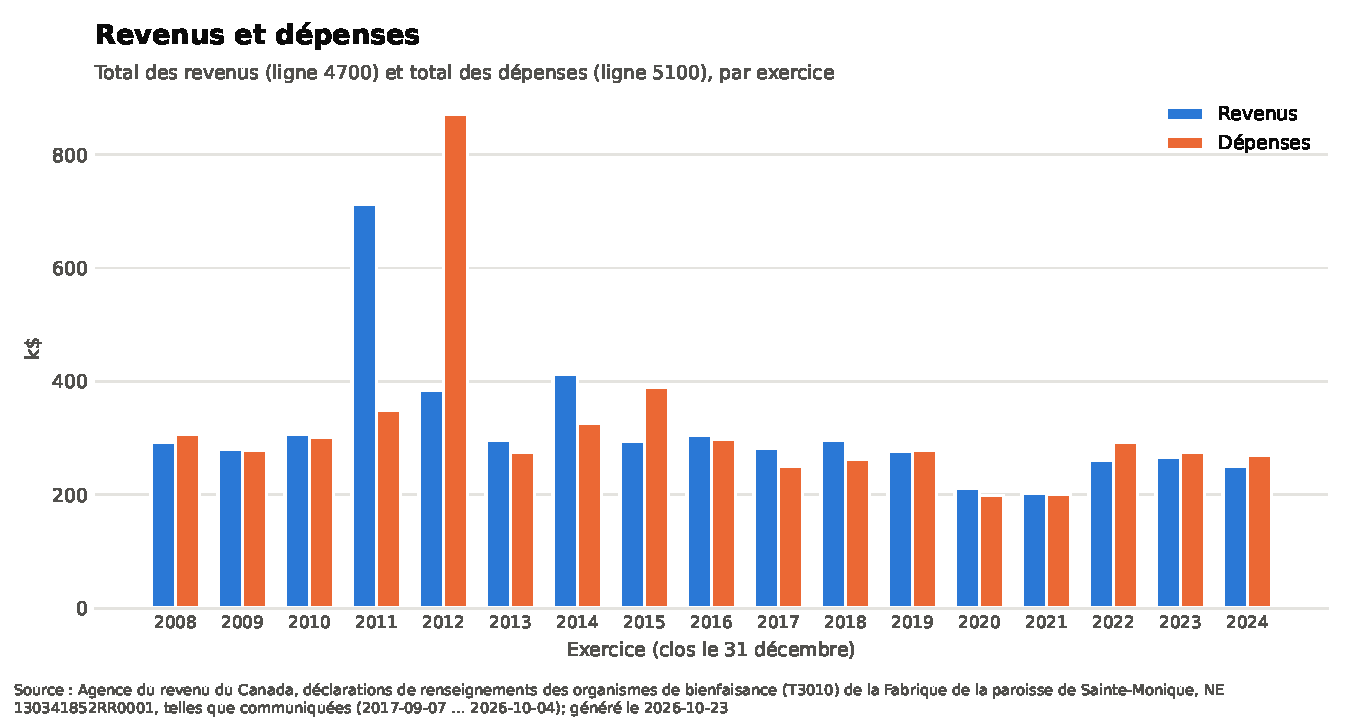
\includegraphics[width=\textwidth]{figures/revenue_and_expenditures_fr.pdf}\end{center}

Le total des revenus (ligne 4700) se situe entre \D{280\,506} (2009) et \D{305\,803} (2010) dans huit des onze années 2008--2018. Les exceptions sont 2011 (\D{711\,793}), 2012 (\D{383\,418}) et 2014 (\D{412\,231}). Le total des dépenses (ligne 5100) se situe entre \D{250\,879} (2017) et \D{305\,884} (2008) dans sept années~; les exceptions sont 2011 (\D{349\,750}), 2012 (\D{871\,127}), 2014 (\D{326\,842}) et 2015 (\D{389\,129}). Les revenus ont dépassé les dépenses en 2009, 2010, 2011, 2013, 2014, 2016, 2017 et 2018~; les dépenses ont dépassé les revenus en 2008 (de \D{13\,966}), 2012 (de \D{487\,709}) et 2015 (de \D{94\,529}).

De 2019 à 2024, le total des revenus est de \D{276\,981} (2019), \D{211\,438} (2020), \D{202\,900} (2021), \D{259\,956} (2022), \D{266\,650} (2023) et \D{250\,718} (2024)~; 2020 et 2021 sont les deux valeurs les plus basses des dix-sept années. Le total des dépenses est de \D{277\,716}, \D{198\,279}, \D{201\,549}, \D{291\,727}, \D{274\,890} et \D{269\,373}. Les dépenses ont dépassé les revenus en 2019 (de \D{735}), 2022 (de \D{31\,771}), 2023 (de \D{8\,240}) et 2024 (de \D{18\,655})~; les revenus ont dépassé les dépenses en 2020 (de \D{13\,159}) et 2021 (de \D{1\,351}). Sur les dix-sept années, les revenus ont dépassé les dépenses dans dix et les dépenses ont dépassé les revenus dans sept.

\subsection{Revenus par ligne}

\begin{center}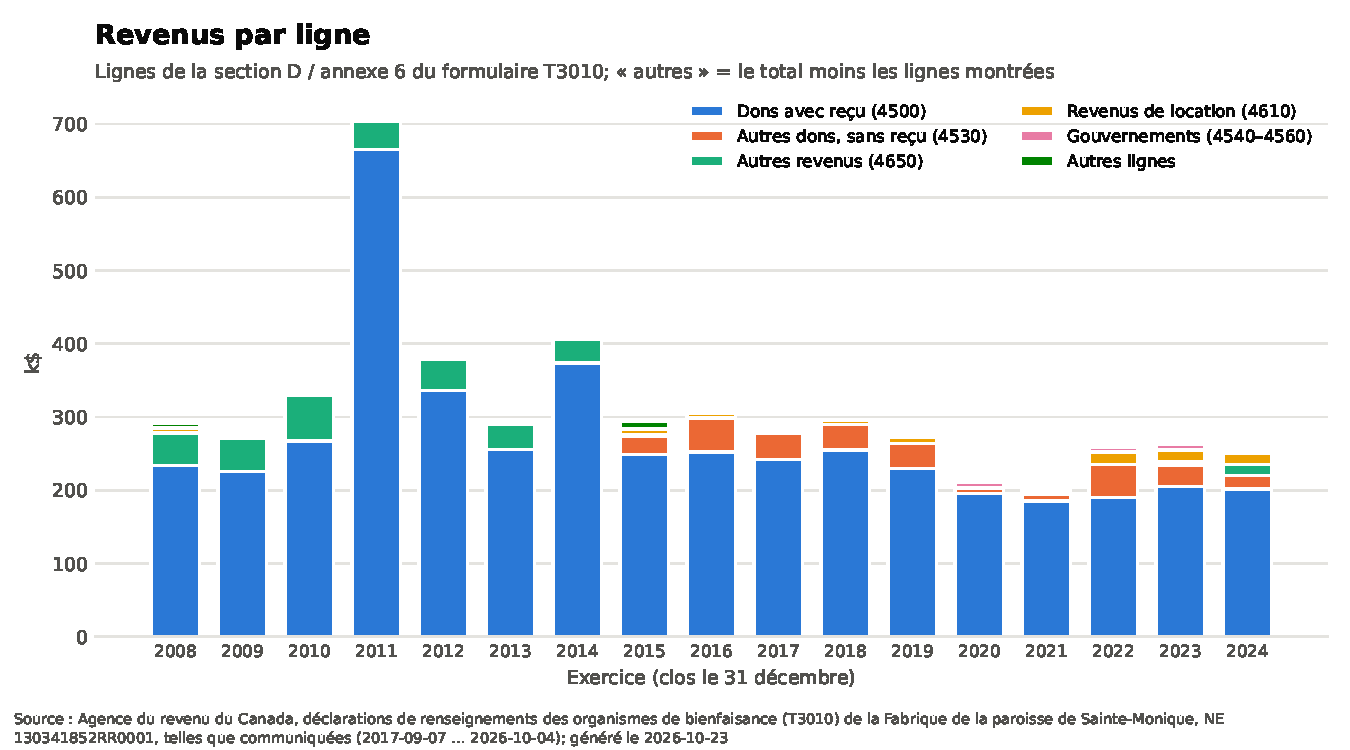
\includegraphics[width=\textwidth]{figures/revenue_by_line_fr.pdf}\end{center}

Les dons avec reçu (ligne 4500) sont la ligne la plus importante chaque année~: de \D{225\,815} à \D{266\,956} en 2008--2010 et 2013--2018 sauf 2014 (\D{373\,427}), et \D{665\,140} en 2011. Les «\,autres revenus\,» (ligne 4650, décrits en 2011 comme messes, funérailles et mariages) vont de \D{32\,913} à \D{63\,217} de 2008 à 2014, puis \D{2\,387} en 2015 et \D{3\,365} en 2017, et sont absents en 2016 et 2018~; à partir de 2015, une ligne vide auparavant, les autres dons sans reçu (4530), porte de \D{24\,600} à \D{46\,244}. Les revenus de location (4610) vont de \D{2\,500} à \D{7\,687} dans les dix années où ils sont présents (aucun en 2017)~; les intérêts et revenus de placements (4580) sont de \D{6\,707} en 2008 et de \D{45} à \D{3\,278} ensuite~; aucun revenu des gouvernements n'est déclaré dans ces années.

À partir de 2019, les dons avec reçu sont de \D{229\,425} (2019), \D{195\,512} (2020), \D{185\,599} (2021), \D{190\,139} (2022), \D{204\,950} (2023) et \D{201\,562} (2024)~; les valeurs de 2020 à 2024 sont les cinq plus basses des dix-sept années. Les autres dons sans reçu (4530) sont de \D{34\,530}, \D{6\,602}, \D{9\,277}, \D{44\,861}, \D{29\,266} et \D{18\,311}. Les revenus de location sont de \D{8\,925} en 2019, \D{1\,175} en 2020 et \D{3\,460} en 2021, puis \D{17\,490}, \D{15\,875} et \D{15\,339} en 2022--2024, au-dessus de chaque année antérieure. Les «\,autres revenus\,» (4650) sont absents de 2019 à 2022, de \D{4\,943} en 2023 (ligne 4655~: «\,recovery of expenses\,») et de \D{15\,506} en 2024 (ligne 4655, telle que déclarée~: «\,Faith First, Virgil lights\,»). Des revenus des gouvernements apparaissent pour la première fois~: \D{3\,781} en 2019 (fédéral \D{1\,636}, provincial \D{2\,145}), \D{7\,448} en 2020, \D{4\,428} en 2021, \D{6\,866} en 2022 (provincial seulement), \D{7\,201} en 2023 et aucun en 2024. Les intérêts et revenus de placements sont de \D{320}, \D{701}, \D{136}, \D{600} et \D{4\,415} de 2019 à 2023 et absents en 2024.

\subsection{La ligne qui nommait messes, funérailles et mariages}\label{sec:4650}

\begin{center}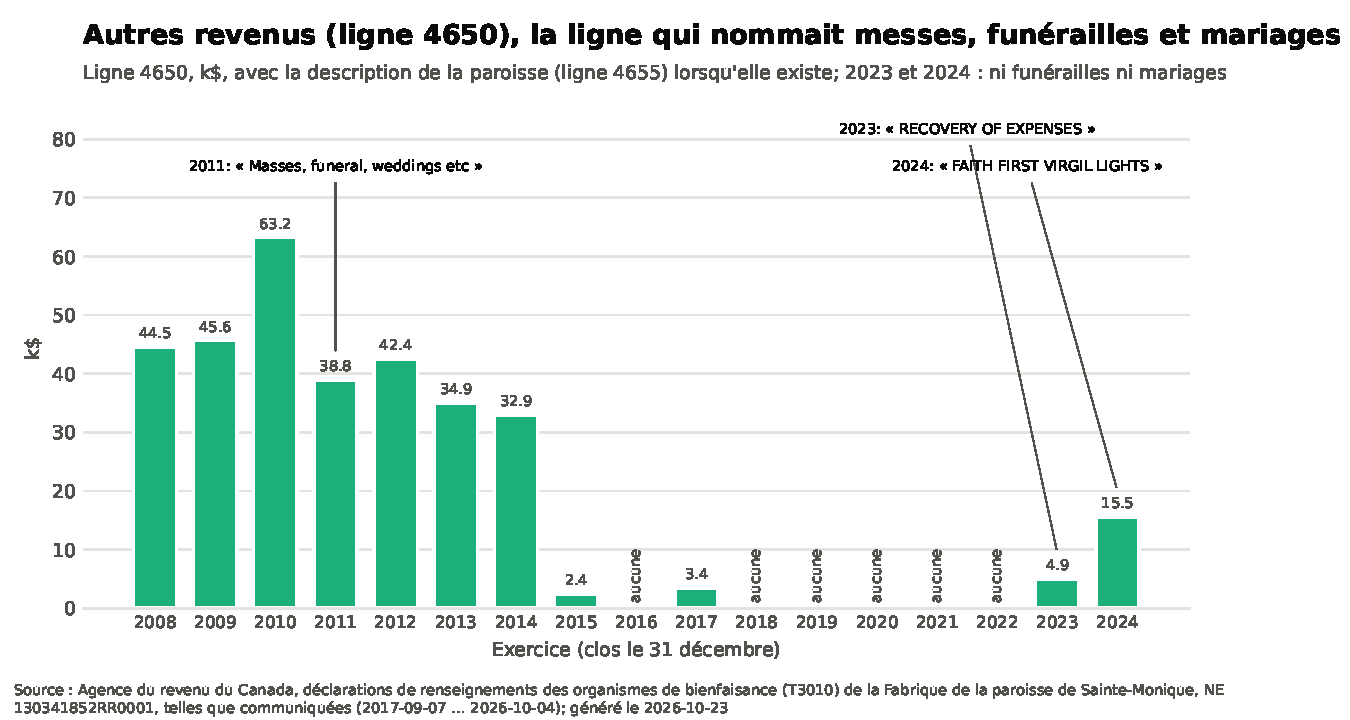
\includegraphics[width=\textwidth]{figures/other_revenue_4650_fr.pdf}\\[-2pt]
{\footnotesize Ligne 4650 par année, avec la description que la paroisse a déclarée à la ligne 4655 lorsqu'elle l'a fait. Les descriptions de 2023 et 2024 (dépenses récupérées~; le programme Faith First et les lampions) ne nomment ni funérailles ni mariages~; seule celle de 2011 le fait.}\end{center}

Une affirmation fréquente dans le débat est que la piste a réduit les revenus de la paroisse tirés des mariages et des funérailles. La déclaration n'a pas de ligne pour les mariages ni pour les funérailles. La ligne la plus proche est la 4650, «\,autres revenus non compris ailleurs\,», que la paroisse a décrite à la ligne 4655 en 2011 comme «\,Masses, funeral, weddings etc\,»~; aucune autre année avant 2023 ne porte de description. Ses valeurs sont de \D{44\,517} (2008), \D{45\,642} (2009), \D{63\,217} (2010), \D{38\,840} (2011), \D{42\,443} (2012), \D{34\,943} (2013) et \D{32\,913} (2014)~; puis \D{2\,387} en 2015, aucune en 2016, \D{3\,365} en 2017, aucune de 2018 à 2022, \D{4\,943} en 2023 (ligne 4655~: «\,recovery of expenses\,») et \D{15\,506} en 2024 (ligne 4655, tel que déclaré~: «\,Faith First, Virgil lights\,», soit le programme de catéchèse des enfants de la paroisse, dont ses bulletins annoncent les séances chaque automne, et les lampions allumés dans l'église~; «\,Virgil\,» pour vigil). Selon les descriptions de la paroisse elle-même, les montants de 2023 et 2024 sur cette ligne sont donc des dépenses récupérées, des frais de programme et des offrandes de lampions, et non des revenus de funérailles ou de mariages~; seule la description de 2011 nomme ceux-ci. L'année où la ligne tombe de \D{32\,913} à \D{2\,387}, 2015, est la première année avec une valeur à la ligne 4530, autres dons sans reçu (\D{24\,600}). Les déclarations ne disent pas sous quelle ligne les revenus des messes, funérailles et mariages sont déclarés depuis 2015.

L'état des revenus et dépenses de la paroisse elle-même pour 2019 et 2020, publié dans son bulletin du 14~novembre 2021, porte une ligne «\,Other income\,» de \D{83\,157} (2019) et \D{66\,260} (2020) avec la note «\,Includes Hall Rentals, bequests, funerals, weddings, etc.\,». Les déclarations de ces deux années ne portent aucune valeur à la ligne 4650, \D{8\,925} et \D{1\,175} en revenus de location (4610), \D{34\,530} et \D{6\,602} en dons sans reçu (4530) et \D{229\,425} et \D{195\,512} en dons avec reçu (4500). Les revenus que la paroisse regroupe comme «\,autres revenus\,» sont donc répartis, dans la déclaration, sur des lignes que celle-ci ne détaille pas davantage.

Le guide de l'ARC pour la déclaration (T4033) définit ainsi les lignes (texte anglais du guide). Ligne 4500~: «\,the total eligible amount of gifts received by the charity during the fiscal period for which official donation receipts have been or will be issued\,». Ligne 4530~: «\,the total amount of all other gifts for which official donation receipts were not issued\,», y compris «\,gifts for which the charity did not issue official donation receipts because it could not identify the donor, such as anonymous gifts\,». Ligne 4630~: revenus «\,from fundraising activities for which official donation receipts were not issued, including the gross amounts from activities carried on by the charity (for example, collection boxes and loose collections)\,». Ligne 4610~: «\,the gross income received or earned by the charity from renting its land and buildings\,», y compris «\,income from leasing out surplus space such as in a church parking lot\,». Ligne 4650~: «\,the total of all other revenue received or earned by the charity that is not already included in the amounts above\,», y compris les remboursements de taxes de vente et la location d'équipement. Une somme versée à l'occasion d'un mariage ou de funérailles peut donc figurer à la ligne 4500 si la paroisse délivre un reçu, à la ligne 4530 si elle la traite comme un don sans reçu, à la ligne 4610 s'il s'agit de la location de la salle ou de l'église, ou à la ligne 4650~; la déclaration ne dit pas laquelle. Le glossaire de l'ARC définit le don comme «\,a voluntary transfer of property without valuable consideration to the donor\,» et admet un avantage au donateur jusqu'à 80~\% du montant sans que le transfert cesse d'être un don.

Pourquoi certains dons sont sans reçu, dans les mots de l'ARC~: à la question de savoir si un organisme enregistré doit délivrer des reçus officiels pour les dons qu'il reçoit, l'ARC répond «\,No. Receipting carries with it a certain administrative burden. Therefore, registered charities may choose to issue receipts according to certain criteria, or they may choose not to issue receipts at all. Some registered charities set minimum donation thresholds for receipting. Others do not provide receipts during certain fundraising events.\,» Un reçu exige aussi un donateur identifié~: l'exemple du guide pour la ligne 4530 est le don anonyme, et les quêtes en espèces vont à la ligne 4630. Pour une paroisse, la quête du dimanche se partage donc entre les enveloppes (avec reçu, ligne 4500) et les espèces (lignes 4530 ou 4630), et une somme donnée lors de funérailles ou d'un mariage reçoit ou non un reçu selon la pratique de la paroisse, que la déclaration ne consigne pas.

Pour la question soulevée dans le débat, le dossier donne donc~: une ligne qui a porté messes, funérailles et mariages de 2008 à 2014, de \D{32\,913} à \D{63\,217} par année, presque vide depuis 2015 pendant qu'une ligne de dons sans reçu apparaissait~; et, pour les années suivantes, trois lignes qui peuvent porter ces revenus sans les isoler, dont la somme est de \D{43\,455} (2019), \D{7\,777} (2020), \D{12\,737} (2021), \D{62\,351} (2022), \D{50\,084} (2023) et \D{49\,156} (2024)~: lignes 4530, 4610 et 4650 additionnées. Les déclarations ne contiennent aucun décompte de mariages ou de funérailles ni aucun revenu attribuable à eux seuls, pour aucune année.

\subsection{Dépenses par ligne}

\begin{center}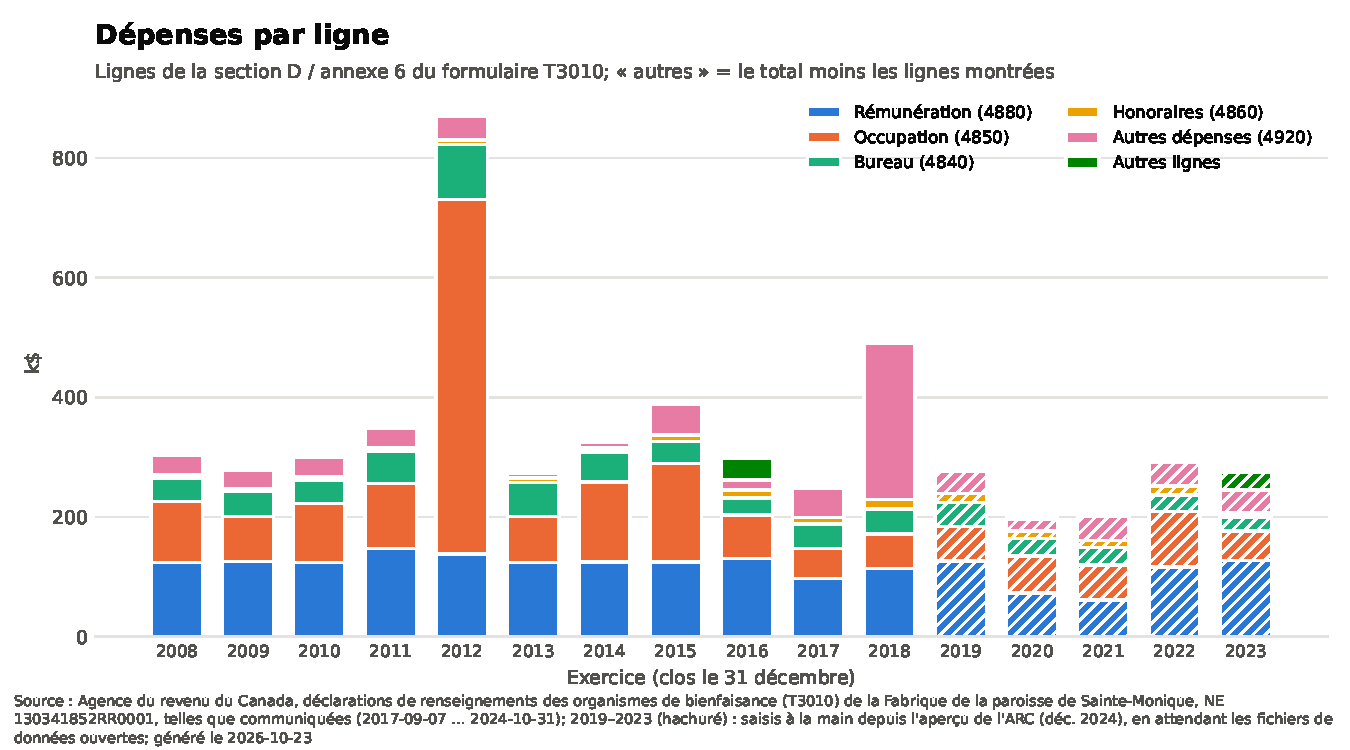
\includegraphics[width=\textwidth]{figures/expenditures_by_line_fr.pdf}\end{center}

La rémunération (ligne 4880) est la ligne de dépenses la plus importante chaque année sauf 2012~: de \D{97\,314} (2017) à \D{147\,183} (2011). Les frais d'occupation (4850) vont de \D{50\,016} (2017) à \D{164\,999} (2015) dans dix années et atteignent \D{592\,737} en 2012, l'année du total le plus élevé. Les frais de bureau (4840) vont de \D{28\,196} à \D{92\,281}~; les honoraires professionnels (4860) de \D{5\,400} à \D{15\,428}~; la ligne «\,toutes les autres dépenses\,» (4920, décrite comme contributions au diocèse et taxes de vente) de \D{7\,245} à \D{50\,844} de 2008 à 2017. La déclaration de 2018 porte \D{261\,865} à la ligne 4920 et le même chiffre à la ligne 5100, et aucune valeur à la ligne 4950.

À partir de 2019, la rémunération est de \D{126\,787} (2019), \D{72\,993} (2020) et \D{61\,370} (2021), les deux valeurs les plus basses de la série, puis \D{116\,820}, \D{127\,217} et \D{143\,000} en 2022--2024~; 2024 est la deuxième valeur la plus élevée après 2011. Les frais d'occupation sont de \D{57\,262}, \D{62\,123}, \D{58\,403}, \D{92\,477}, \D{49\,802} et \D{57\,319}~; 2023 est la valeur la plus basse des dix-sept années. Les frais de bureau passent de \D{40\,598} en 2019 à \D{11\,456} en 2024, la valeur la plus basse de la série~; les honoraires professionnels sont de \D{14\,736}, \D{12\,373}, \D{11\,995}, \D{15\,015}, \D{6\,000} et \D{6\,239}. La ligne «\,toutes les autres dépenses\,» est de \D{37\,634}, \D{19\,776}, \D{40\,604}, \D{39\,200}, \D{38\,757} et \D{22\,820}, décrite à la ligne 4930 comme éducation de la foi, taxes de vente et contribution diocésaine (2019), taxes de vente et contribution diocésaine (2020--2022), «\,worship expenses\,» (2023) et «\,Faith First, worship, Virgil lights\,» (2024, tel que déclaré). Deux lignes portent des valeurs importantes en 2023 et 2024 pour la première fois~: permis, adhésions et cotisations (4830), \D{25\,080} et \D{22\,219} après \D{35} à \D{37} de 2019 à 2022, et fournitures et biens achetés (4891), \D{3\,983} en 2023. La déclaration de 2024 est la première avec des dons aux donataires reconnus (5050), \D{5\,822}, de sorte que le total des dépenses (\D{269\,373}) dépasse la ligne 4950 (\D{263\,551}) de ce montant~; dans toutes les autres années où les deux lignes sont présentes, elles sont égales à deux dollars près.

\subsection{Actif par ligne}

\begin{center}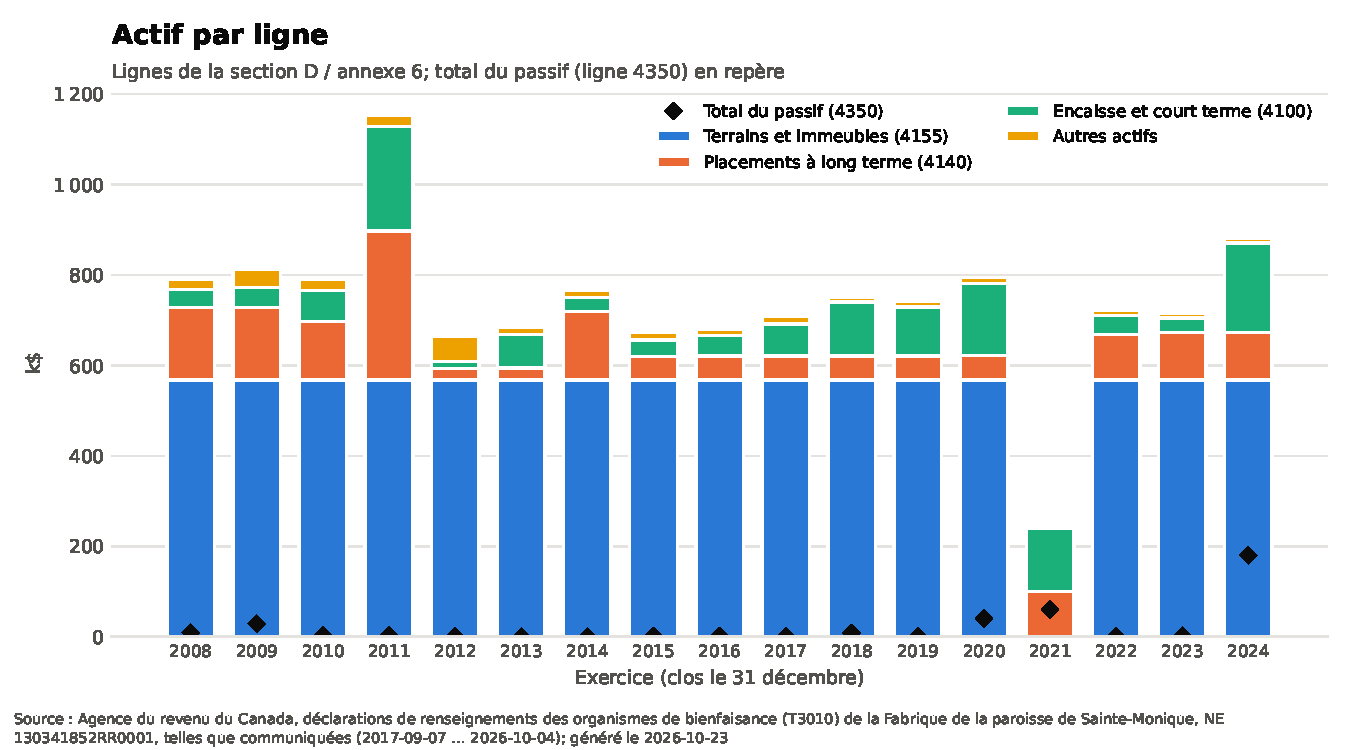
\includegraphics[width=\textwidth]{figures/assets_by_line_fr.pdf}\end{center}

Les terrains et immeubles sont de \D{567\,643} chaque année de 2009 à 2018 (\D{567\,642} en 2010 et 2013). Les placements à long terme (4140) sont de \D{160\,000} en 2008--2009, \D{130\,000} en 2010, \D{330\,000} en 2011, \D{26\,124} en 2012, \D{26\,385} en 2013, \D{151\,941} en 2014 et de \D{52\,436} à \D{53\,307} à partir de 2015. L'encaisse et les placements à court terme (4100) vont de \D{14\,765} (2012) à \D{231\,051} (2011)~; ils sont de \D{119\,181} en 2018. Le total du passif (4350, égal aux comptes créditeurs, ligne 4300, chaque année) va de \D{8} à \D{28\,711}.

À partir de 2019, les terrains et immeubles sont de \D{567\,643} en 2019, 2020, 2022, 2023 et 2024~; la déclaration de 2021 ne porte aucune valeur à la ligne 4155, et son total de l'actif, \D{246\,995}, est la somme de ses autres lignes d'actif. Le total de l'actif est de \D{741\,843} (2019), \D{794\,350} (2020), \D{723\,035} (2022), \D{716\,315} (2023) et \D{881\,634} (2024), le plus élevé depuis 2011. Les placements à long terme sont de \D{53\,626} et \D{54\,326} en 2019--2020 et de \D{100\,000} à \D{105\,600} à partir de 2021. L'encaisse et les placements à court terme sont de \D{108\,466}, \D{159\,574}, \D{139\,938}, \D{42\,378}, \D{31\,528} et \D{197\,111}~; 2024 est la deuxième valeur la plus élevée de la série après 2011. Le total du passif est de \D{1\,414} (2019), \D{40\,762} (2020), \D{60\,000} (2021~: comptes créditeurs \D{40\,000} et revenus reportés \D{20\,000} à la ligne 4310, la seule année avec cette ligne), \D{268} (2022), \D{2\,123} (2023) et \D{180\,109} (2024), le plus élevé des dix-sept années~; dans les autres années, le total du passif égale les comptes créditeurs.

\section{Comparaison avec les autres paroisses du secteur}\label{sec:peers}

Un changement dans les chiffres d'une paroisse ne se lit que contre ce que les paroisses voisines ont fait les mêmes années. Le fichier d'identification du jeu de données 2024 de l'ARC donne chaque organisme enregistré avec son adresse~; les paroisses catholiques («\,fabriques\,») dont le code postal commence par H3T, H3X, H3Z, H4A, H4B, H4V ou H4W, soit Côte-des-Neiges, Snowdon, Westmount, Notre-Dame-de-Grâce et Côte-Saint-Luc, sont douze outre Sainte-Monique~: Notre-Dame-des-Neiges, Saint-Kevin, Saint-Antonin, Saint-Malachie, Saint-Léon, Ascension of Our Lord, Notre-Dame-de-Grâce, Saint Augustine of Canterbury (ces deux-là à une même adresse dans le fichier 2024), Saint-Raymond, Saint-Ignace-de-Loyola, Sainte-Catherine-de-Sienne et Saint-Richard (\texttt{derived/peer\_parishes.csv}). Le script \texttt{derived/fetch\_peer\_parishes.py} garde leurs lignes du fichier financier de chaque année de 2015 à 2024 dans \path{raw/open-canada-peers/<année>/} (\texttt{SOURCES.tsv} comme ci-dessus)~; les treize sont présentes les dix années. \texttt{derived/peer\_comparison.py} écrit la table longue (\texttt{peer\_comparison\_long.csv}), la table en indices et la table des variations, et les trois graphiques ci-dessous.

Deux mesures sont comparées. Les dons sont les deux lignes de dons additionnées, 4500 et 4530, parce que la part avec reçu varie d'une paroisse à l'autre~: en 2024 elle est de 92~\% à Sainte-Monique et de 39~\% à 100~\% chez les douze autres, de sorte qu'aucune des deux lignes seule n'est comparable. Le total des revenus est la ligne 4700. Chaque paroisse est mise en indice de sa propre moyenne 2017--2019, pour que des paroisses de tailles très différentes (revenus totaux de \D{105\,748} à \D{768\,204} en 2024) se lisent sur une même échelle~; la courbe de la paroisse étudiée est tracée par-dessus les douze autres, leur médiane et leur moitié centrale.

\begin{center}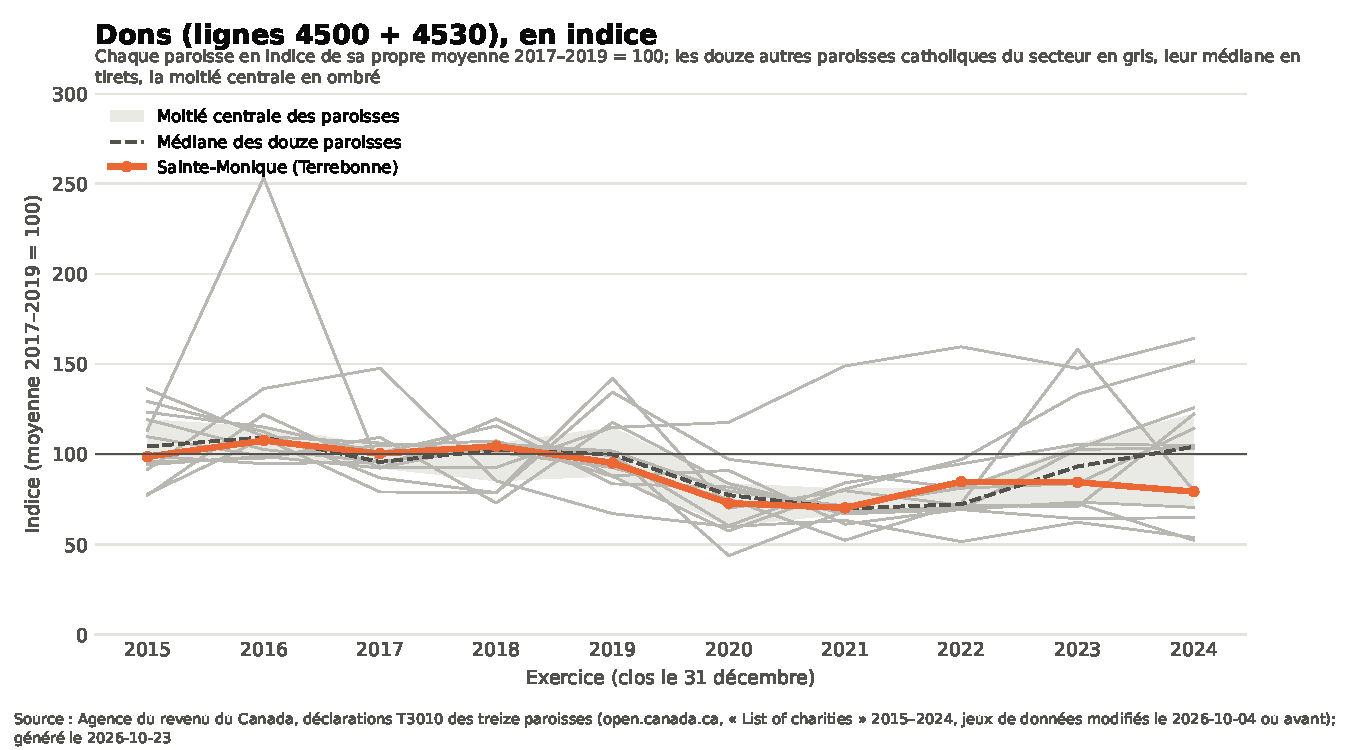
\includegraphics[width=\textwidth]{figures/peers_gifts_index_fr.pdf}\end{center}
\begin{center}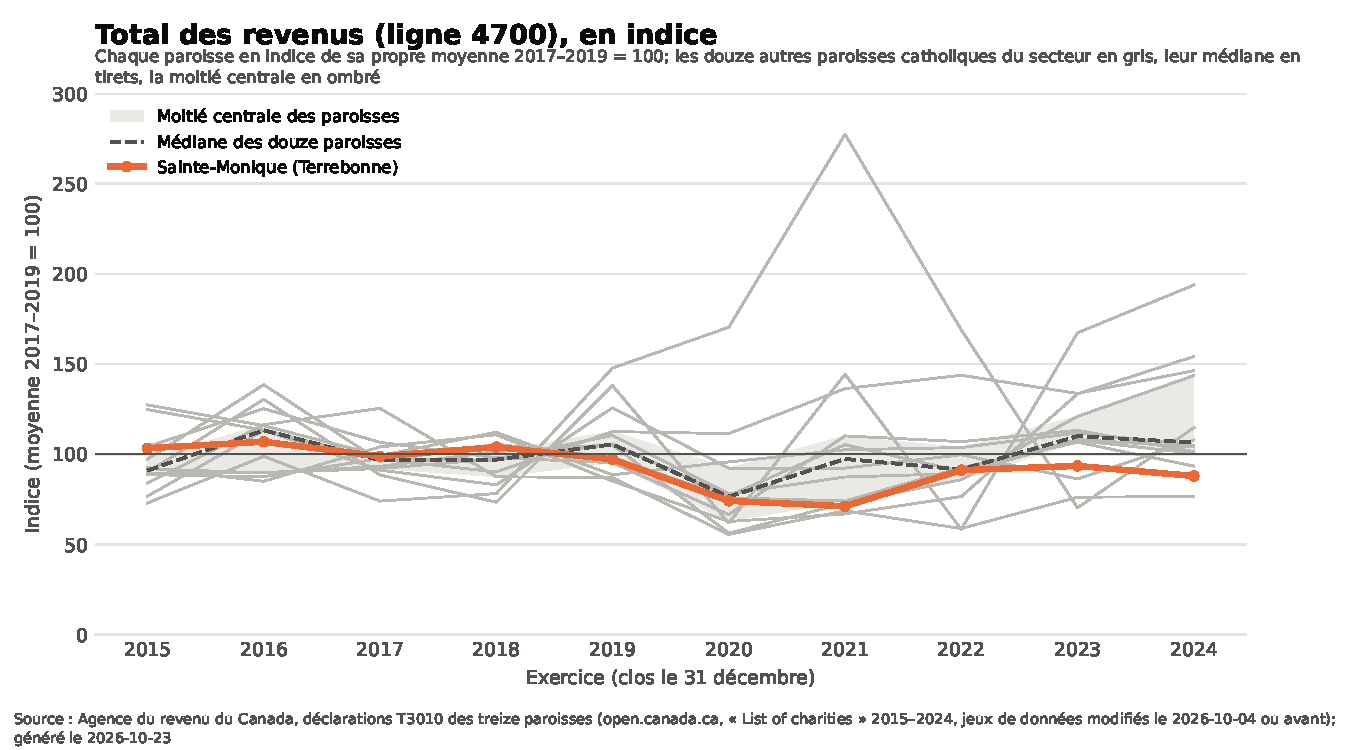
\includegraphics[width=\textwidth]{figures/peers_revenue_index_fr.pdf}\end{center}
\begin{center}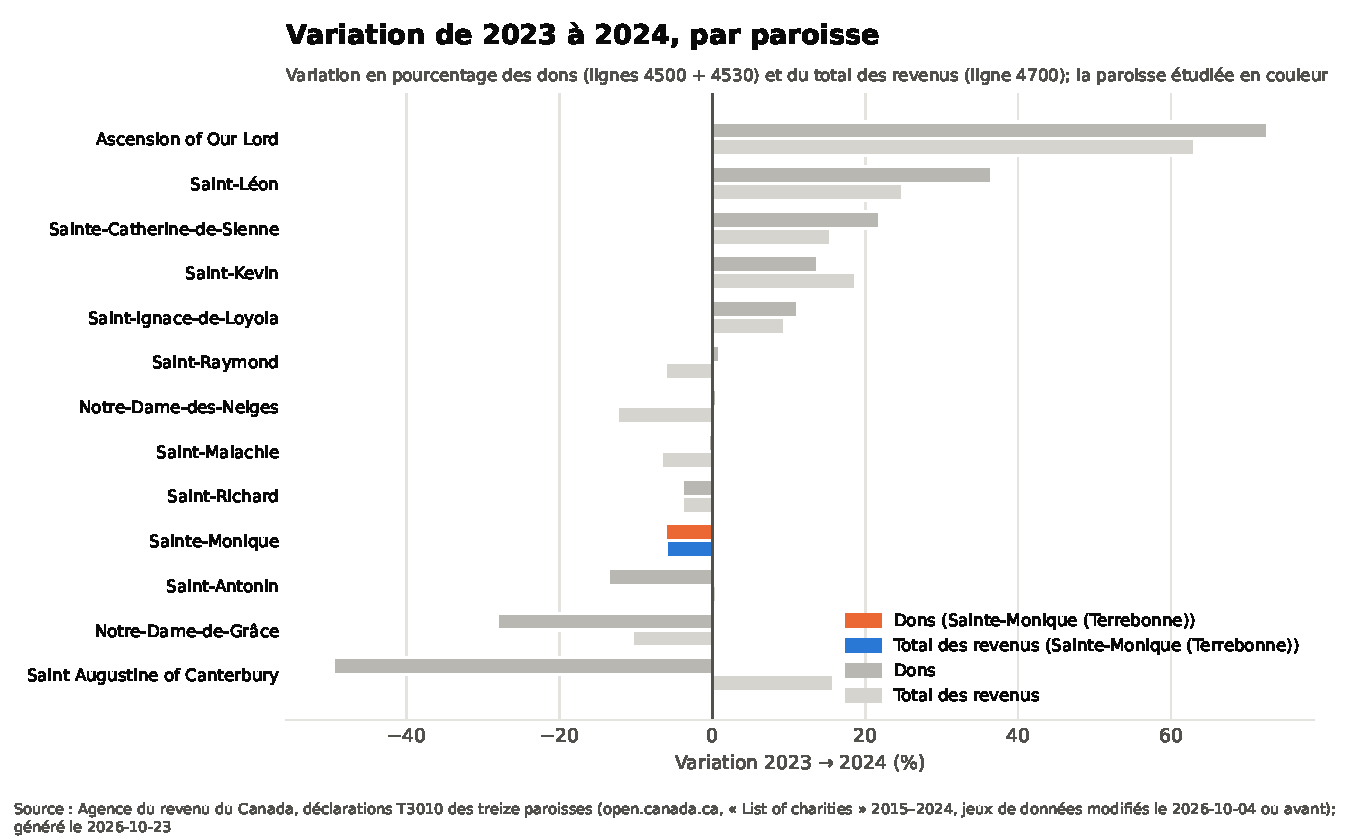
\includegraphics[width=\textwidth]{figures/peers_change_2024_fr.pdf}\end{center}

Ce que montre la comparaison. Sur les dons, Sainte-Monique est à 79 en 2024 par rapport à sa moyenne 2017--2019, la médiane des paroisses voisines à 104 et leur moitié centrale entre 71 et 122~; la paroisse était au-dessus de la médiane en 2022 (85 contre 72), en dessous en 2023 (84 contre 93) et plus bas encore en 2024. Sur le total des revenus, 88 en 2024 contre une médiane de 106 et une moitié centrale de 101 à 144~; au niveau de la médiane en 2022 (91 contre 92), en dessous en 2023 (94 contre 110) et en 2024. De 2023 à 2024, les dons de la paroisse ont baissé de 6,1~\% et son total des revenus de 6,0~\%~; chez les douze voisines, les dons ont varié d'une médiane de $+$0,8~\% (moitié centrale de $-$11,2 à $+$19,9~\%~; sept en hausse, cinq en baisse, dont trois de plus que Sainte-Monique) et le total des revenus d'une médiane de $+$5,0~\% (moitié centrale de $-$6,5 à $+$18,0~\%~; sept en hausse, cinq en baisse). Par rapport à la moyenne 2022--2023, les dons 2024 de la paroisse sont de 6,3~\% inférieurs et ses revenus de 4,8~\%, là où les médianes des voisines sont de $+$5,8 et $+$5,1~\%~; sur chaque mesure la paroisse se classe neuvième à onzième des treize. L'écart entre la variation de la paroisse et la médiane des voisines est donc d'environ sept points sur les dons et onze sur les revenus, à l'intérieur de la dispersion des variations des voisines elles-mêmes, dont la moitié centrale s'étend sur 31 et 25 points et l'étendue complète de $-$50 à $+$73~\%.

\subsection{Seuil de détection~: quelle ampleur de changement se détacherait}\label{sec:threshold}

La variation d'une année à l'autre observée avant la piste fixe ce que ce dossier peut détecter. Deux plans sont jaugés~: la paroisse contre sa propre histoire (plan A~: la variation en pourcentage d'une ligne d'une année à la suivante), et la paroisse contre ses voisines (plan B~: la variation de la paroisse moins la variation médiane des douze voisines la même année). Pour chacun, le bruit est l'écart-type des huit variations d'avant la piste, 2015--2016 à 2022--2023, calculé deux fois~: sur les huit, et sur les cinq qui excluent les trois transitions marquées par la pandémie (vers 2020, vers 2021 et vers 2022). Le seuil est fixé à deux écarts-types~: une variation au-delà serait inhabituelle au niveau d'environ 5~\% si les variations étaient normales et indépendantes~; avec huit observations, c'est une jauge, pas un test. La piste a couvert sept des douze mois de 2024, de sorte qu'un effet annuel de la piste paraît dans la déclaration de 2024 aux sept douzièmes de sa taille~; l'effet annuel détectable en 2024 est le seuil multiplié par douze septièmes. Une année complète (la déclaration de 2025) est détectable au seuil lui-même~; la moyenne de deux années complètes au seuil divisé par $\sqrt{2}$. Le script est \texttt{derived/detection\_threshold.py}~; sa table~:

\begin{center}\resizebox{\textwidth}{!}{\begin{tabular}{@{}lllrrrrrrr@{}}\toprule
Mesure & Plan & Bruit & $n$ & ET des variations (\%) & Seuil, 2 ET (\%) & Effet annuel détectable en 2024 (\%) & Avec une année complète (\%) & Avec deux années complètes (\%) & Observé 2024 (\%) \\\midrule
Dons (4500 + 4530) & paroisse seule & les huit variations d'avant la piste & 8 & 13 & 26 & 45 & 26 & 18 & $-$6,1 \\
Dons (4500 + 4530) & paroisse seule & sans les trois transitions COVID & 5 & 7,4 & 15 & 26 & 15 & 10 & $-$6,1 \\
Dons (4500 + 4530) & paroisse moins la médiane des voisines & les huit variations d'avant la piste & 8 & 7,8 & 16 & 27 & 16 & 11 & $-$6,9 \\
Dons (4500 + 4530) & paroisse moins la médiane des voisines & sans les trois transitions COVID & 5 & 7,2 & 14 & 25 & 14 & 10 & $-$6,9 \\
Total des revenus (4700) & paroisse seule & les huit variations d'avant la piste & 8 & 15 & 29 & 50 & 29 & 21 & $-$6,0 \\
Total des revenus (4700) & paroisse seule & sans les trois transitions COVID & 5 & 6,0 & 12 & 21 & 12 & 8,5 & $-$6,0 \\
Total des revenus (4700) & paroisse moins la médiane des voisines & les huit variations d'avant la piste & 8 & 16 & 33 & 56 & 33 & 23 & $-$11 \\
Total des revenus (4700) & paroisse moins la médiane des voisines & sans les trois transitions COVID & 5 & 9,5 & 19 & 33 & 19 & 14 & $-$11 \\
\bottomrule\end{tabular}
}\end{center}

Lu sur les dons, plan B sans les transitions COVID, la combinaison la plus favorable~: un effet de la piste aurait dû retrancher environ 25~\% des dons annuels de la paroisse pour se détacher en 2024~; l'écart observé à la médiane des voisines est de $-$7 points. Lu sur la paroisse seule avec les huit variations, la moins favorable~: environ 45~\%. Deux années complètes après la piste, au même bruit, ramèneraient l'effet détectable à environ 10 à 18~\% des dons.

Ce qui limite la comparaison. Douze paroisses font un petit ensemble, et plusieurs portent des mouvements qui leur sont propres dans ces années~: l'une a des autres revenus de \D{400\,000} à \D{700\,000} en 2020--2022 et plus depuis, une autre voit ses dons diminuer de moitié en 2024 pendant que son total des revenus monte de 72~\%, deux partagent une adresse. Les déclarations ne disent rien de ce qui s'est passé chez aucune d'elles (travaux, fusions, clergé, campagnes), ni à Sainte-Monique, dont la campagne de financement 2024--2025 (\D{163\,858} recueillis, selon son bulletin du 21~décembre 2025) paraîtra dans les lignes de dons de 2024 et 2025. La comparaison dit où se situent les chiffres 2024 de la paroisse parmi ceux de ses voisines~; elle ne dit pas pourquoi.

\section{Les états de la paroisse elle-même, à côté des déclarations}\label{sec:statements}

La paroisse a publié des états financiers dans ses bulletins hebdomadaires~: un état mensuel (quêtes du dimanche et en ligne du mois, revenus et dépenses cumulés depuis janvier, solde) en 2017, 2018, 2019 et janvier 2020~; un bilan et un état des revenus et dépenses de 2020 à côté de 2019, approuvés par les marguilliers le 11~octobre 2021 et publiés le 14~novembre 2021~; un tableau des douze mois de 2022 (5~février 2023) et un rapport sur janvier à septembre 2022 (6~novembre 2022)~; et les mois de janvier à mars 2023 (16 et 23~avril 2023). Aucun bulletin d'avril 2023 au 18~octobre 2026 ne porte d'état financier~; le seul tableau financier ultérieur est un sommaire des collectes de fonds 2024--2025 (21~décembre 2025, ci-dessous). Les bulletins sont sur le site web de la paroisse et ne sont pas reproduits ici, parce qu'ils nomment des personnes~; les chiffres des états le sont, dans \texttt{derived/parish\_statements\_monthly.csv}, lus dans les bulletins à l'œil~: 46 mois et fins d'année avec des chiffres, chacun avec la date et le nom de fichier du bulletin et une note sur chaque particularité (un en-tête qui nomme la mauvaise année, un chiffre imprimé sur la mauvaise ligne et corrigé la semaine suivante, trois soldes qui ne correspondent pas aux lignes au-dessus à quelques dollars près, un déficit imprimé sans ses parenthèses, et un rapport trimestriel de novembre 2022 dont les quêtes en ligne s'ajoutent aux chiffres mensuels là où le tableau annuel de février 2023 dit qu'elles y sont incluses).

\subsection{Recoupement~: les états de fin d'année et les déclarations}

\begin{center}\small\begin{tabular}{@{}lrrrrrrl@{}}\toprule
Exercice & État : revenus & État : dépenses & Déclaration 4700 & Déclaration 5100 & Écart, revenus & Écart, dépenses & État publié le \\\midrule
2018 & 296\,581 & 264\,954 & 296\,399 & 261\,865 & 182 & 3\,089 & 2019-01-20 \\
2019 & 276\,981 & 277\,716 & 276\,981 & 277\,716 & 0 & 0 & 2021-11-14 \\
2020 & 211\,438 & 198\,279 & 211\,438 & 198\,279 & 0 & 0 & 2021-11-14 \\
2022 & 259\,957 & 291\,726 & 259\,956 & 291\,727 & 1 & $-$1 & 2023-02-05 \\
\bottomrule\end{tabular}
\end{center}

Là où les deux existent, l'état de fin d'année de la paroisse et la déclaration concordent au dollar près pour 2019, 2020 et 2022~; pour 2018, l'état du 20~janvier 2019 (\D{296\,581} et \D{264\,954}) et la déclaration (\D{296\,399} et \D{261\,865}) diffèrent de \D{182} et \D{3\,089}. Le bilan de 2020 publié en novembre 2021 concorde au dollar près avec les lignes d'actif et de passif de la déclaration, au 31~décembre 2020 comme au 31~décembre 2019~: encaisse \D{159\,574} et \D{108\,466} (ligne 4100), placements \D{54\,326} et \D{53\,627} (4140), montants à recevoir \D{4\,598} et \D{2\,385} (4120), frais payés d'avance \D{8\,209} et \D{9\,723} (4170), terrains et immeubles \D{567\,643} (4155), passif \D{40\,762} et \D{1\,414} (4350). Le total des dépenses de l'état de 2020, \D{198\,279}, est net d'un remboursement de subvention salariale de \D{12\,263} (SSUC), et la ligne 5100 de la déclaration porte le même chiffre net.

\subsection{Ce que les états ajoutent aux déclarations}

\begin{center}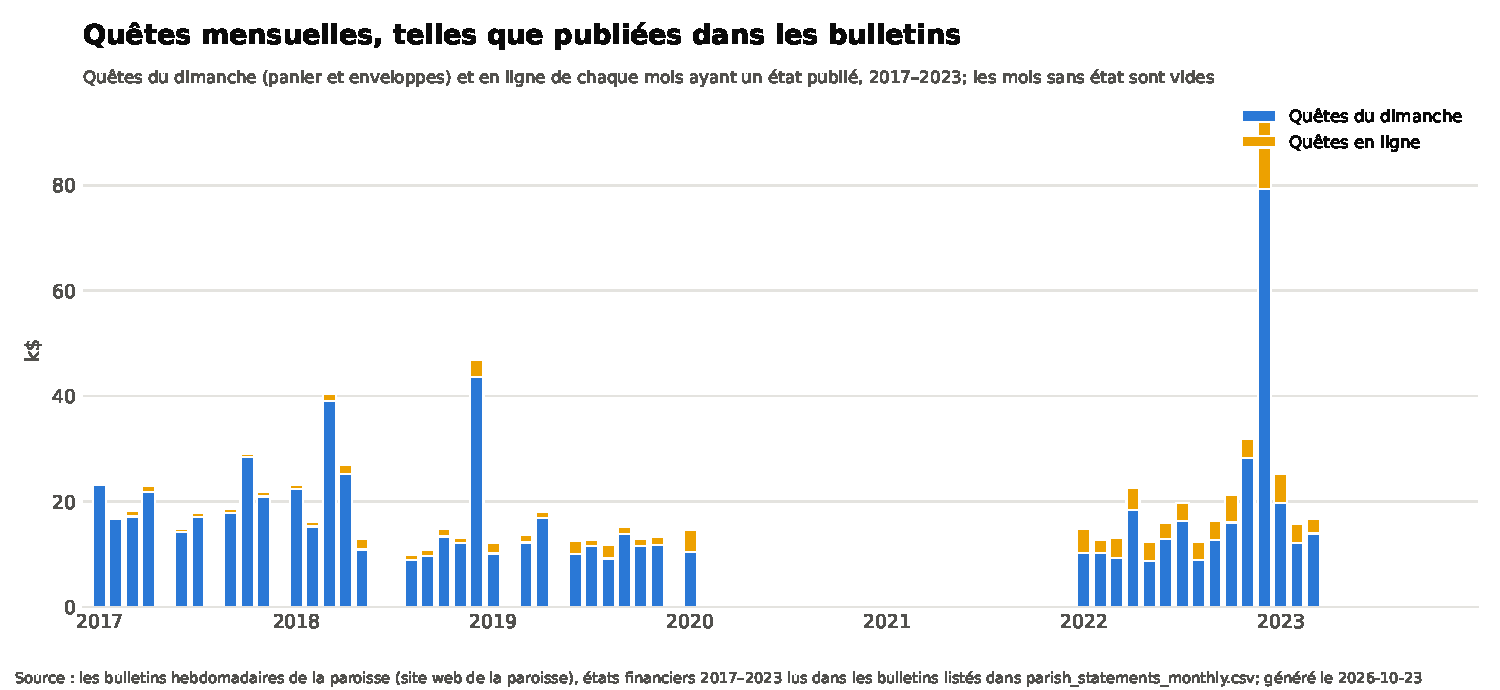
\includegraphics[width=\textwidth]{figures/parish_monthly_collections_fr.pdf}\end{center}
\begin{center}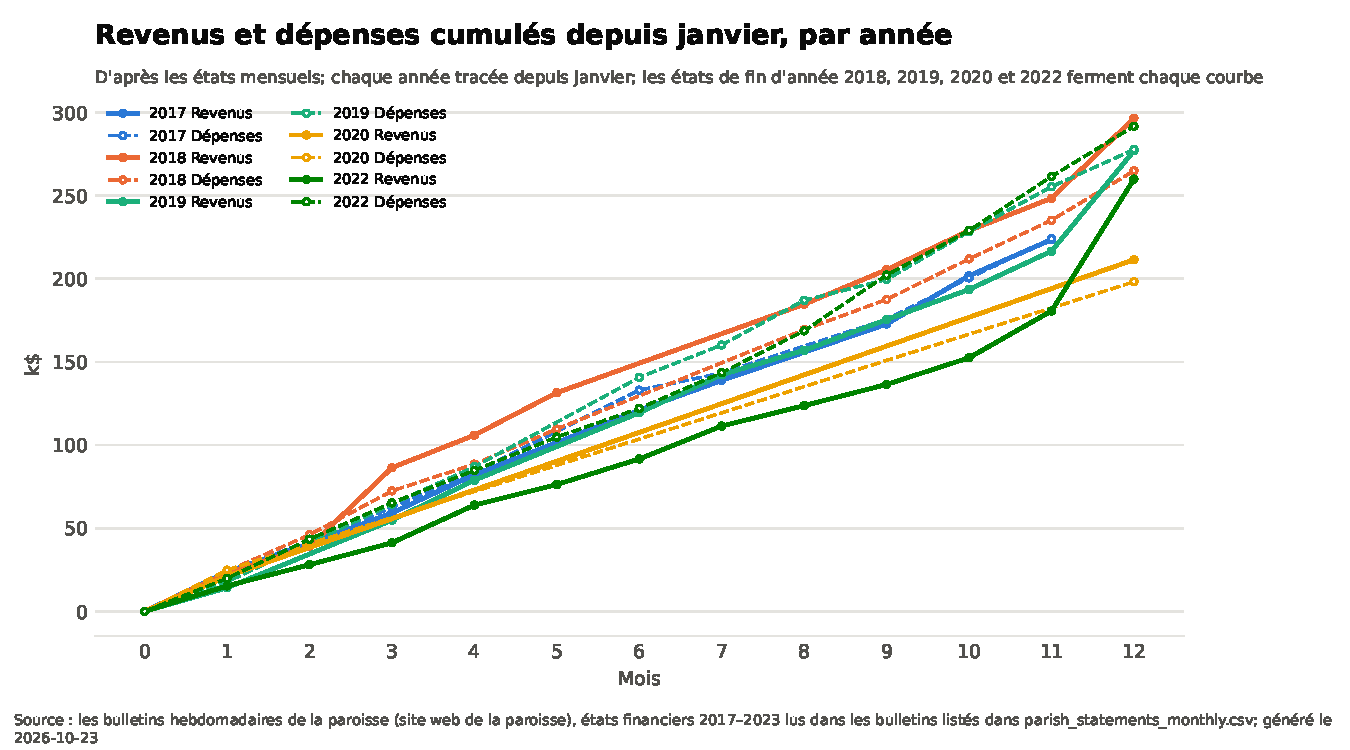
\includegraphics[width=\textwidth]{figures/parish_ytd_fr.pdf}\end{center}

Trois choses que la déclaration ne porte pas. D'abord, la ventilation des revenus dans les catégories de la paroisse~: pour 2019 et 2020, quêtes de fin de semaine \D{154\,575} et \D{119\,872}, offrandes pour l'entretien \D{13\,849} et \D{6\,118}, autres offrandes spéciales \D{25\,400} et \D{19\,188}, et «\,other income\,» \D{83\,157} et \D{66\,260}, dont la note se lit «\,Includes Hall Rentals, bequests, funerals, weddings, etc.\,»~; les deux lignes de dons de la déclaration pour ces années (\D{263\,955} et \D{202\,114}) dépassent les offrandes de l'état (\D{193\,824} et \D{145\,178}) de \D{70\,131} et \D{56\,936}, de sorte que l'essentiel de ce que la paroisse comptabilise comme autres revenus est déclaré comme dons (section~\ref{sec:4650}). L'état de 2020 porte aussi la subvention salariale et un prêt de \D{30\,000} du Compte d'urgence pour les entreprises canadiennes (CUEC), remboursable avant la fin de 2022, que la déclaration ne montre que dans le passif. Ensuite, le mois~: les quêtes du dimanche vont de \D{10\,000} à \D{17\,000} par mois en 2019 (\D{43\,662} en décembre 2018, le mois le plus fort de la série), les quêtes en ligne de \D{500} à \D{2\,500} avant 2020 et de \D{2\,600} à \D{5\,500} en 2022--2023~; le tableau de 2022 montre un déficit dès janvier, qui atteint \D{80\,813} fin novembre et se referme à \D{31\,770} après un décembre à \D{79\,277} de quêtes. Enfin, le premier trimestre de 2023~: des quêtes de \D{25\,217}, \D{15\,778} et \D{16\,753} contre des dépenses de \D{28\,293}, \D{20\,640} et \D{26\,106}, un déficit de \D{17\,291} au 31~mars 2023, derniers chiffres mensuels publiés par la paroisse.

Pour la question de cette note, la série s'arrête quatorze mois avant l'aménagement de la piste~; aucun chiffre mensuel n'existe pour 2024 ni 2025, et le profil mensuel qu'il faudrait pour séparer les mois d'avant et d'après juin 2024 n'est pas dans le dossier public.

\subsection{Ce que disent les bulletins depuis l'arrêt des états}

Tous les bulletins de l'archive du site web de la paroisse ont été lus pour cette note~: 519 numéros, de mai 2014 au 18~octobre 2026. Quatre constats. Les états n'ont pas repris~: du 30~avril 2023 au 18~octobre 2026, aucun bulletin ne porte d'état mensuel ou annuel, de bilan, de budget ni de chiffre de déficit~; une offre d'emploi de septembre 2023 compte la production des états mensuels et cumulés parmi les tâches d'un comptable. Le compte rendu que la paroisse fait elle-même de ses finances pour 2024--2026 est une campagne de financement pour son 75\textsuperscript{e} anniversaire, «\,Preserving the Past, Building the Future\,», pour «\,the repairs and maintenance of our Rectory and Church\,»~: un arbre de donateurs aux feuilles gravées à partir d'octobre 2024~; un tableau du 21~décembre 2025 donnant, pour 2024--2025, \D{163\,858} recueillis (événements de 2024 \D{35\,605}, de 2025 \D{28\,674}, collecte générale \D{36\,986}, arbre des donateurs \D{62\,593}), \D{13\,687} de dépenses, \D{149\,516} restants, et \D{25\,955} de réparations majeures en 2025 (une infiltration d'eau au presbytère, \D{14\,955}) avec \D{123\,561} restants~; en avril 2026, la campagne est dite menée «\,over the past three years\,», avec l'engagement d'un paroissien de verser \D{25\,000} en contrepartie des contributions~; en octobre 2026, la restauration des colonnes de l'église est annoncée terminée et les fenêtres à l'arrière de l'église remplacées. Les lignes de dons des déclarations de 2024 et 2025 comprennent donc une campagne d'immobilisations que la déclaration ne sépare pas des dons ordinaires. Un événement porte le nom de la paroisse dans le sien~: les bulletins des 3, 10 et 17~novembre 2024 annoncent que «\,the Save St.~Monica's Support Group with the St.~Monica's Fundraising Committee will be holding a rally in the church basement, Sunday November 24th immediately after the 11am mass\,», avec quatre numéros de scène, entrée libre, «\,a donation at the door\,» et des reçus fiscaux pour les dons de plus de 25~\$~; les annonces n'énoncent aucune raison au rassemblement, le nom du groupe n'apparaît dans aucun autre bulletin, aucun bulletin ne rapporte ce que le rassemblement a recueilli, et le tableau des collectes de décembre 2025 donne les événements de 2024 en un seul total (\D{35\,605} recueillis). Aucun bulletin ne mentionne la piste cyclable~: dans les 519 numéros, les mots bike, bicycle et cyclist n'apparaissent qu'une fois, dans une chronique de février 2019 sur une «\,église verte\,» suggérant un support à vélos et le covoiturage, et «\,Terrebonne\,» n'apparaît que dans l'adresse de la paroisse~; aucun bulletin n'attribue une difficulté à la piste ni aux travaux de la rue. Compté sur les numéros publiés après l'aménagement de la piste~: dans les 117 bulletins datés du 1\textsuperscript{er}~juillet 2024 au 18~octobre 2026, il n'y a aucune référence à la piste cyclable, aucune à des difficultés financières qui lui seraient liées, et aucune à des difficultés de stationnement~; le mot «\,parking\,» y apparaît trois fois, en février 2026, pour un stationnement gratuit lors d'un cours tenu hors de la paroisse. Ce silence n'est pas celui d'un bulletin confiné aux choses spirituelles~: les mêmes numéros portent des avis pratiques et civiques, dont l'arrangement de stationnement d'octobre 2023, le poste de comptable à pourvoir en septembre 2023, les comptes de collecte et les réparations rapportés ci-dessus, des campagnes de Développement et Paix demandant aux paroissiens de signer pour une loi fédérale (octobre--novembre 2024) et une pétition (mars 2025), les élections des marguilliers, et, le 19~octobre 2025, un avis intitulé «\,Municipal Election -- Make Your Voice Heard!\,» disant que «\,local officials make decisions that affect housing, snow removal, parks, safety, and community programs\,» et que les résidents de Côte-des-Neiges--Notre-Dame-de-Grâce doivent être «\,consulted and heard on local issues that matter\,», avec les dates du scrutin. Les bulletins ne donnent pas non plus de compte de la communauté~: les décès n'y paraissent que par des avis occasionnels et dans les intentions de messe, les baptêmes et mariages seulement comme consignes permanentes du secrétariat, et la seule série qu'ils portent est le nombre de jeunes confirmés ou faisant leur première communion chaque printemps (confirmations~: 28 en 2014, 38 en 2015, 21 en 2016, 24 en 2017, 33 en 2018, 35 en 2019, 28 en 2022, 25 en 2023, 23 en 2024, 17 en 2025, 18 en 2026~; premières communions~: 24, 23, 25 en 2014--2016, 30 en 2019, 19 en 2022, 29 en 2023, 22 en 2024, 14 en 2026), une mesure du programme de catéchèse plutôt que de l'assistance~; la lettre du curé du 7~septembre 2025 dit que «\,our Mass attendance remained steady\,» pendant l'été, sans chiffre.

\subsection{La page Facebook de la paroisse}

La page Facebook officielle de la paroisse («\,St.~Monica's Parish Montreal\,», 814 abonnés) a été interrogée le 23~octobre 2026 avec la recherche de publications de la page, pour bike, lane, path, parking, piste, Terrebonne, petition, rally, «\,save St.~Monica\,» et le nom du centre voisin. Quatre publications concernent la piste. Trois datent de la piste temporaire de 2020~: le 25~juillet 2020, «\,an appeal to our parishioners to take note that if this bike path proceeds as planned, there will be no parking on either side of Terrebonne from Belmore to Oxford. Many of our parishioners are elderly or have reduced mobility. There will be no place to park for people attending weddings or funerals, not to mention Sunday Mass\,», avec un lien vers une pétition et une invitation à écrire à la mairesse d'arrondissement et au conseiller de district (sept réactions, quatre commentaires, deux partages)~; le 31~août 2020, un lien vers le formulaire de questions du conseil municipal sur «\,the upcoming bike lane extension from Madison to Cavendish\,»~; le 4~septembre 2020, un lien vers le formulaire de questions du conseil d'arrondissement pour la séance du 8~septembre, où «\,a motion proposed … for its removal\,» devait être entendue, avec la remarque que «\,as I pointed out at the Press Conference, the church is deeply concerned about the environment and wants our streets to be safe and healthy for everyone\,», suivie des consignes d'un comité de citoyens pour les questions et les courriels. La quatrième est la seule publication depuis la piste de 2024~: le 14~août 2024, la page a partagé un article du Religion News Service du 13~août 2024, «\,Would Jesus park in a bike lane? For Philadelphia churches, it's a real question\,», avec la légende «\,An article relevant to many of our parish communities in Montreal!\,» (une réaction, un commentaire). L'article n'est pas une protestation contre les pistes cyclables~: il rapporte que la Tenth Presbyterian Church de Philadelphie a renoncé à son permis de stationner dans une piste cyclable le dimanche matin après dix-huit semaines de manifestations de cyclistes, son pasteur exécutif disant aux fidèles que les voisins «\,see us as self-centered\,», que la Philadelphia Ethical Society avait déplacé son stationnement vers un parc voisin, «\,the right thing to do\,», que l'Old Pine Street Church avait appuyé les pistes dès le départ et obtenu un stationnement du dimanche une rue plus loin, et que cinq des sept congrégations du parcours avaient trouvé des solutions~; une directrice d'association cycliste y parle de se rencontrer «\,in the middle\,». Le partage mettait donc sous les yeux des paroissiens un récit d'églises s'accommodant d'une piste cyclable. Depuis l'aménagement de la piste protégée, ce partage est le seul commentaire public officiel de la paroisse sur les pistes cyclables~; ses publications de 2020 sur la piste temporaire, à laquelle elle s'opposait, accompagnaient déjà cette opposition de la déclaration que l'église «\,is deeply concerned about the environment and wants our streets to be safe and healthy for everyone\,». Aucune publication ne mentionne l'arrangement de stationnement de 2023, le rassemblement de novembre 2024, ni un effet financier de la piste. Sur le stationnement~: le 15~octobre 2023, la paroisse a annoncé que «\,through the kindness of the MacKay Center, our next door neighbour, we have secured additional parking spaces for those attending Mass at St.~Monica's Church during the weekends on Saturdays and Sundays throughout the year\,», dans l'aire de stationnement latérale du Centre, avec des vignettes de tableau de bord pour «\,a minimum one time donation of \$5.00\,»~; l'avis a été répété jusqu'au 3~décembre 2023 et n'apparaît plus ensuite. L'arrangement précède la piste de sept mois.

\section{Ce que le dossier ne contient pas}

La déclaration de l'exercice 2025 et des suivants~: l'ARC a publié le fichier de chaque année tard dans l'année suivante, et aucun jeu de données 2025 n'était sur le portail le 23~octobre 2026 (le script et la table d'identifiants sont prêts). Les bulletins eux-mêmes, qui nomment des personnes~; les chiffres de leurs états sont à la section~\ref{sec:statements}. Les déclarations ne donnent que des totaux par année civile~: rien ici ne sépare 2024 en mois avant et après l'aménagement de la piste.

\section{Reproduction}

\texttt{python3 derived/build.py} reconstruit chaque table, chaque graphique et les deux notes à partir de \texttt{raw/}~; \texttt{python3 derived/fetch\_open\_data.py} ajoute les extraits de données ouvertes des années marquées \emph{to\_fetch} dans \texttt{open\_canada\_datasets.csv} (\texttt{--search} liste les jeux de données du portail, \texttt{--list} les fichiers d'un jeu, \texttt{--extract} prend un fichier téléchargé à la main). La date de construction et les dates «\,as of\,» des données sont imprimées sur chaque graphique~; la note porte sa version en pied de page.

\end{document}
